\documentclass[12pt]{article}
\usepackage{amsmath}
\usepackage{graphicx}
\usepackage{cite}
\date{}
\begin{document}

\tableofcontents
\pagebreak

\section{Introduction}

The work focuses on the relationships between dependent binomial variables, with the intention of modelling K-stage binomial processes and offering improved decision rules for MAB style problems.

So far we have assumed each 'lever' to be a website. Though models could just as well apply to a particular placement or creative.

We hope that the models can be further expanded to include a more complex hierarchy, for example, campaign-site-placement. Or could dependencies on for example, fixed effect regressors for creative or user category.

We provide:
\begin{itemize}
	\item A set of models for dealing with dependent binomial data, including data generation functions.
	\item A set of diagnostic tests for assessing the validity of each model for a novel dataset.
	\item A framework for assessing the usefulness of each model against relevant loss functions for RTB problems.
	\item Decision rules to optimise the explore-exploit trade off in RTB campaigns.
\end{itemize}


\section{Data}

We have 3 vector valued random variables. The ith index represents the values for site domain i for a particular lineitem. In the context on a MAB problem, each index represents a lever. The variables are defined as:
\begin{itemize}
	\item \textbf{n} - number of impressions served over given time period
	\item \textbf{c} - number of clicks on impressions over same time period 
	\item \textbf{a} - number of acquisitions over same time period
\end{itemize}

TODO - bring in relevant sections of EDA document here.

\section{Models}
We define 7 models to fit the data, ultimately intending to model acquisitions.

We start with simple binomial model (m1), then look to beta binomial (m3) to deal with over-dispersion. We then bring in intermediate clicks, hoping these can offer more information on the likelihood of future acqusitions. We find that clicks provide no information on acquisitions unless there is a dependency between p and q. We consider both a cluster model as well as a correlation model to model dependency between p and q.

\subsection{Model 1 - Single Binomial} 
All levers are assumed to have the same payoff function. A useful baseline model. We assume a uniform Beta prior so that the MAP estimate of r is equivlanet to the MLE and is also an unbiased estimator. We gain as much information about lever 1 by looking at lever 2 as by looking at lever 1.

  \begin{align}
	a_i \sim Bin(r,n_i) \\
	\pi(r) = Beta(1,1)
  \end{align}

\subsection{Model 2 - Independent Binomials} 
We assume that each lever has a completely independent payoff function. There is no information to be gained about lever 1 by looking at lever 2.

  \begin{align}
	a_i \sim Bin(r_i,n_i) \\
	\pi(r_i) = Beta(1,1)
  \end{align}

\subsection{Model 3 - Beta-binomial} 
Useful if data is over dispersed for a binomial model. Here we assume a hierarchical model where the conversion rate for each lever is sampled from a Beta distribution with common $\alpha$, $\beta$ parameters across all levers. In a sense, this model lies somewhere between model 1 and model 2, in that data about lever 1 gives us some information about lever 2 via inference of $\alpha$, $\beta$ parameters. 

  \begin{align}
	a_i \sim Bin(r_i,n_i) \\
	r_i \sim Beta(\alpha,\beta) \\
	\pi(\alpha) = Unif(0,10000) \\
	\pi(\beta) = Unif(0,10000)
  \end{align}

\subsection{Model 4 - Beta-binomial plus clicks} 
Since acquisitions are rare events, we try to gain more information about a lever be modelling the click-through-rate separately from the conversions. Similarly to model 3, CTR and CVR have a hierarchical model.

  \begin{align}
	a_i \sim Bin(q_i,c_i) \\
	c_i \sim Bin(p_i,n_i) \\
	q_i \sim Beta(\alpha_q,\beta_q) \\
	p_i \sim Beta(\alpha_p,\beta_p) \\
	\pi(\alpha_q) = Unif(0,10000) \\
	\pi(\beta_q) = Unif(0,10000) \\
	\pi(\alpha_p) = Unif(0,10000) \\
	\pi(\beta_p) = Unif(0,10000) 
  \end{align}

When p and q are independent of each other, $a_i$ has distribution $Bin(p_iq_i,n)$ and $p_iq_i$ has distribution $Beta(a_i,n_i - a_i)$ (see 'Do Clicks Matter' for proof). This makes it equivalent to model 3 with different priors. The intuition here is that clicks are not informative - as much as they increase our belief in click through rate, they decrease our belief in the acquisition rate.

\subsection{Model 5 - 2 cluster Binomial} 

Useful for comparison against model 6.

\subsection{Model 6 - 2 cluster Beta-binomial }

Model 4 assumed that CTR and CVR are independent. Experience suggests that levers tend to perform well on both CTR and CVR or poorly on both. In other words, there tend to be 'clusters' of good and bad levers. Model 5 attempts to capture this with a beta-binomial mixture model. We use priors to bias one cluster towards being the poor performer, this helps avoid 'index switching' complications with model fitting. 
 
 \begin{align}
	a_i \sim Bin(q_i,c_i) \\
	c_i \sim Bin(p_i,n_i) \\
	k \sim Bern(h) 
\end{align}
	\[ 
	q_i \sim 
  	\begin{cases}
		Beta(\alpha_{q0},\beta_{q0}) & \quad \text{if k is 0}\\
		Beta(\alpha_{q1},\beta_{q1}) & \quad \text{if k is 1}
	\end{cases}
	\]
	\[
	p_i \sim 
  	\begin{cases}
		Beta(\alpha_{p0},\beta_{p0}) & \quad \text{if k is 0}\\
		Beta(\alpha_{p1},\beta_{p1}) & \quad \text{if k is 1}\\
	\end{cases}
	\]

 \begin{align}
	\pi(h) = Unif(0,1) \\
	\pi(\alpha_{q0}) = Gamma(1,2) \\
	\pi(\beta_{q0}) = Gamma(1,2) \\
	\pi(\alpha_{p0}) = Gamma(1,2) \\
	\pi(\beta_{p0}) = Gamma(1,2) \\
	\pi(\alpha_{q1}) = Unif(0,10000) \\
	\pi(\beta_{q1}) = Unif(0,10000) \\
	\pi(\alpha_{p1}) = Unif(0,10000) \\
	\pi(\beta_{p1}) = Unif(0,10000)
\end{align}

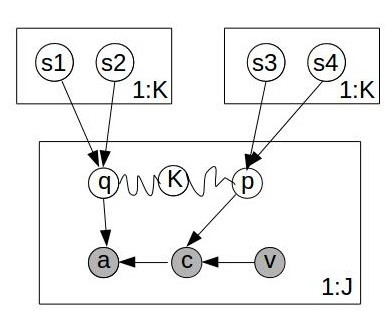
\includegraphics{GraphMod.jpg}

\subsection{Model 7 - Correlated Beta-binomial }

'Bacon With Your Eggs? Applications of a New Bivariate Beta-Binomial Distribution'
'The Use of a Correlated Binomial Model for the Analysis of Certain Toxicological Experiments'
Lee - 'Properties and Applications of the Sarmanov Family of Bivariate Distributions'

As an alternative to model 6, where rate prediction will change abruptly between clusters, we look for a model where q can vary smoothly as a function of p.

We use a relatively unused binomial correlation model, discussed in 'Bacon With Your Eggs? Applications of a New Bivariate Beta-Binomial Distribution'. 

\section{Diagnostic testing}

We take the approach of starting with a simple model and run further tests to decide whether there is evidence to expand the model. 

Where possible we prefer tests with strong theoretical backing, e.g. LR. As model complexity rises it becomes harder to rely on these. We use information criteria and posterior validation.

\subsection{test 1} A frequentist style goodness of fit test designed to assess whether data can be well explained with simple binomial model 1. We use the binomial approximation to the Normal and perform pearson chisq on the residuals. This only holds for large n, so we group the small n values to test whether (together) they share the same mean.

Benefits are that we can have a composite alternative hypothesis, downside is the approximation used. Could be improved by Yates' corerction. TODO - approximation fails for p as rate is very small.

'Goodness-of-Fit Issues in Toxicological Experiments Involving Litters of Varying Size'

\subsection{test 2}

Assuming we reject model 1, we try LR test to see if data is better modelled using beta-binomial. Testing null hypothesis against all others is difficult. LR test has the benefit of being 'most powerful' for comparing 2 point hypotheses, so is a good choice assuming we are happy using ML point hypotheses. If we were willing to specify priors on parameters, we could turn this in to a Bayes factor test.

TODO - compare ratio value to alpha, or do chisq on deviances?

Although this test can show whether Model 3 is better, it can not show whether it is 'good'. This paper has excellent review of goodness-of-fit tests for beta-binomial model:
'Bootstrap goodness-of-fit test for the beta-binomial model'

We use both VGAM and Stan package to get ML estimates for beta-binomial.

\subsection{test 3}

LR test Model 1 vs Model 5 - 1 cluster binomial vs 2 cluster binomial. 

This is a cheap - 'are there clusters between median values' test. 

\subsection{test 4}

Assuming we reject null in test 2, due to some form of over dispersion, we check if can extend this to 2 cluster model with another LR test. Obviously we could keep testing for additional clusters. A more general approach could be to define prior penalizing large number of clusters and use VB or Gibbs to find posterior.

This is a cheap - 'are there clusters between median values' test. 


\subsection{test 5}

Use AIC and BIC for comparison between Model 6 and Model 7. These models aren't nested.

\subsection{Posterior predictive checks}

Similar to the goodness of fit checks, these let us compare our model against observed data. First can use the generating functions to visuallly compare.

\subsubsection{Bayesian p-values}

If we can choose a scalar test statistic, we can produce a p value of realized statistic versus model theoretic probably of the statistic being more extreme than that. Not an obvious candidate.

\subsubsection{Chi-square GoF}

Possibly very useful, need to be careful about the validity of the approximation given some small n.

\section{ Performance testing - static loss functions }

The previous diagnostic tests can help us build a probability model. Ultimately, we are interested in making optimal decisions with a certain loss function. 

We look at the distribution of realized loss functions with k-fold cross validation. And compare the Advance data under each of our proposal models, and benchmark this against the results of the generated data.

We define 4 loss functions:
\begin{enumerate}
	\item Posterior likelihood of realized CVR. 
	\item Difference in conversion rate between estimated top site and true top site.
	\item Volume weighted difference in realized CVR (relates closely to budget wasted). 
	\item Vol weighted MSE.
\end{enumerate}
\section{Results}

\subsection{Correlation measures}

% latex table generated in R 3.0.2 by xtable 1.7-3 package
% Wed Jul 23 18:50:50 2014
\begin{table}[ht]
\centering
\begin{tabular}{rlrrrrrrrr}
  \hline
 & g & Cor & IWC & logIWCc & RankCor & items & imps & glmcoef & glmsignif \\ 
  \hline
1 & m1 & -0.03 & -0.00 & -0.01 & 0.01 & 1681 & 12946112 & 0.12 & 0.00 \\ 
  2 & m\_1023111 & -0.07 & 0.03 & 0.10 & 0.20 & 191 & 23228621 & -0.03 & 0.19 \\ 
  3 & m3 & -0.07 & -0.02 & -0.13 & -0.09 & 364 & 13079687 & -0.10 & 0.01 \\ 
  4 & m5 & 0.14 & 0.05 & 0.37 & 0.27 & 324 & 12815129 & 0.76 & 0.00 \\ 
  5 & m6 & 0.03 & 0.04 & 0.23 & 0.05 & 319 & 12743695 & 0.22 & 0.00 \\ 
   \hline
\end{tabular}
\end{table}


\subsection{Diagnostic tests}

TODO - cluster test fails to identify model 5.
TODO - vgam library has problems fitting non betabinom cluster data.
% latex table generated in R 3.0.2 by xtable 1.7-3 package
% Wed Jul 23 18:51:42 2014
\begin{table}[ht]
\centering
\begin{tabular}{rlrrrl}
  \hline
 & g & test1\_BinomGoF & test2\_BinomVsBetaBinom & test3\_2ClustBinom & test4\_2ClustBetaBinom \\ 
  \hline
1 & m1 & 1.00 & 1.00 & 1.00 & Error \\ 
  2 & m\_1023111 & 0.00 & 0.00 & 1.00 & Error \\ 
  3 & m3 & 0.00 & 0.00 & 1.00 & Error \\ 
  4 & m5 & 0.00 & 0.00 & 1.00 & Error \\ 
  5 & m6 & 0.00 & 0.00 & 0.00 & 0 \\ 
   \hline
\end{tabular}
\end{table}

\section{Conclusions}

\begin{itemize}
	\item Need to use log values of p.
	\item Clustering based on $a_i$ creates false correlations.
	\item Clustering based on c does not create false correlations.
	\item Using c greater than 0, correlations do not show up. But become stronger for c gt 1, c gt 2. This is because it reduces the noise of all the small-n zero and one values.
	\item Filter based on realized CTR is no use as it does not help with (3). Needs a correlation measure which properly accounts for likelihood weight of response - closest thing is glm.
	\item Binomial GLM does the best job of (4), though does not consider error in dependent variable.
\end{itemize}

\pagebreak

\section{ Simulation testing - Model 4}

\subsection{Test harness}

A simulation test harness was set up to simulate MAB trials. Custom policies were run in the harness and assessed against a regret function. We define regret as the difference in r between chosen arm and optimal arm (TODO add notation).

\begin{enumerate}
	\item Experimenter defines a bivariate Beta prior distribution parameterized by alpha and beta values for p and q.
	\item This prior is then used as a generative model to sample a set of 'true' p and q values for each arm.
	\item Each strategy is provided with the prior information and must infer the true values of p and q. The test harness calls on the strategy to return an arm number. The test harness then draws a single sample from a distribution using the true p and q values for this arm. The result is a tuple $(acquisition,click,view)$. The strategy is given this result so that it may update it's knowledge. The mean regret for the strategy is also updated.
	\item Step 3 is repeated for a set number of rounds i.e. the time horizon.
	\item Steps 2, 3 and 4 are looped 100 times so that we can calculate mean regret. Standard error for the mean values is estimated using a bootstrap method.
\end{enumerate}

\subsection{Strategies}

\begin{description}
	\item[ts clicks] Each arm is initialized with a beta prior using the alpha and beta values for p. Arms are chosen using Thompson sampling based on the probability of each arm having maximum p. The algorithm seeks to optimize clicks only, though regret is still calculated in same way.
	\item[ts both] Each arm is initialized with beta prior for both p and q. Arms are chosen using Thompson sampling based on the probability of each arm having maximum r value (i.e. pq). Since the distribution of pq does not in general have an analytic form, we use sampling. The priors on p and q are updated in the usual way.
	\item[ts acqs] The strategy only looks at acquisitions per view, ignoring clicks. Since the Beta priors on p and q do not directly translate in to a Beta prior on r, we estimate the parameters of a Beta prior for r using the mean and variance of p and q. This new Beta prior is updated in the usual way with acquisitions and views.
\end{description}

\subsection{Validation}

We run a set of validation checks to make sure we are not favouring one strategy in some extrinsic way - such as a more informative prior or more accurate posterior sampling.

\begin{enumerate}
	\item  We give p a point prior at value 1. With this, we expect to see the same performance from ts acqs and ts both. ts clicks should select arms arbitrarily.
	\item  We give q a point prior at value 1. With this, we expect to see the same performance from all 3 strategies as they are all 'learning' click rate.
	\item  We give both p and q flat priors. We expect to see the same performance from ts acqs and ts both as our analysis shows this is a special case, equivalent to modelling acquisitions only.
\end{enumerate}

\subsection{Results}

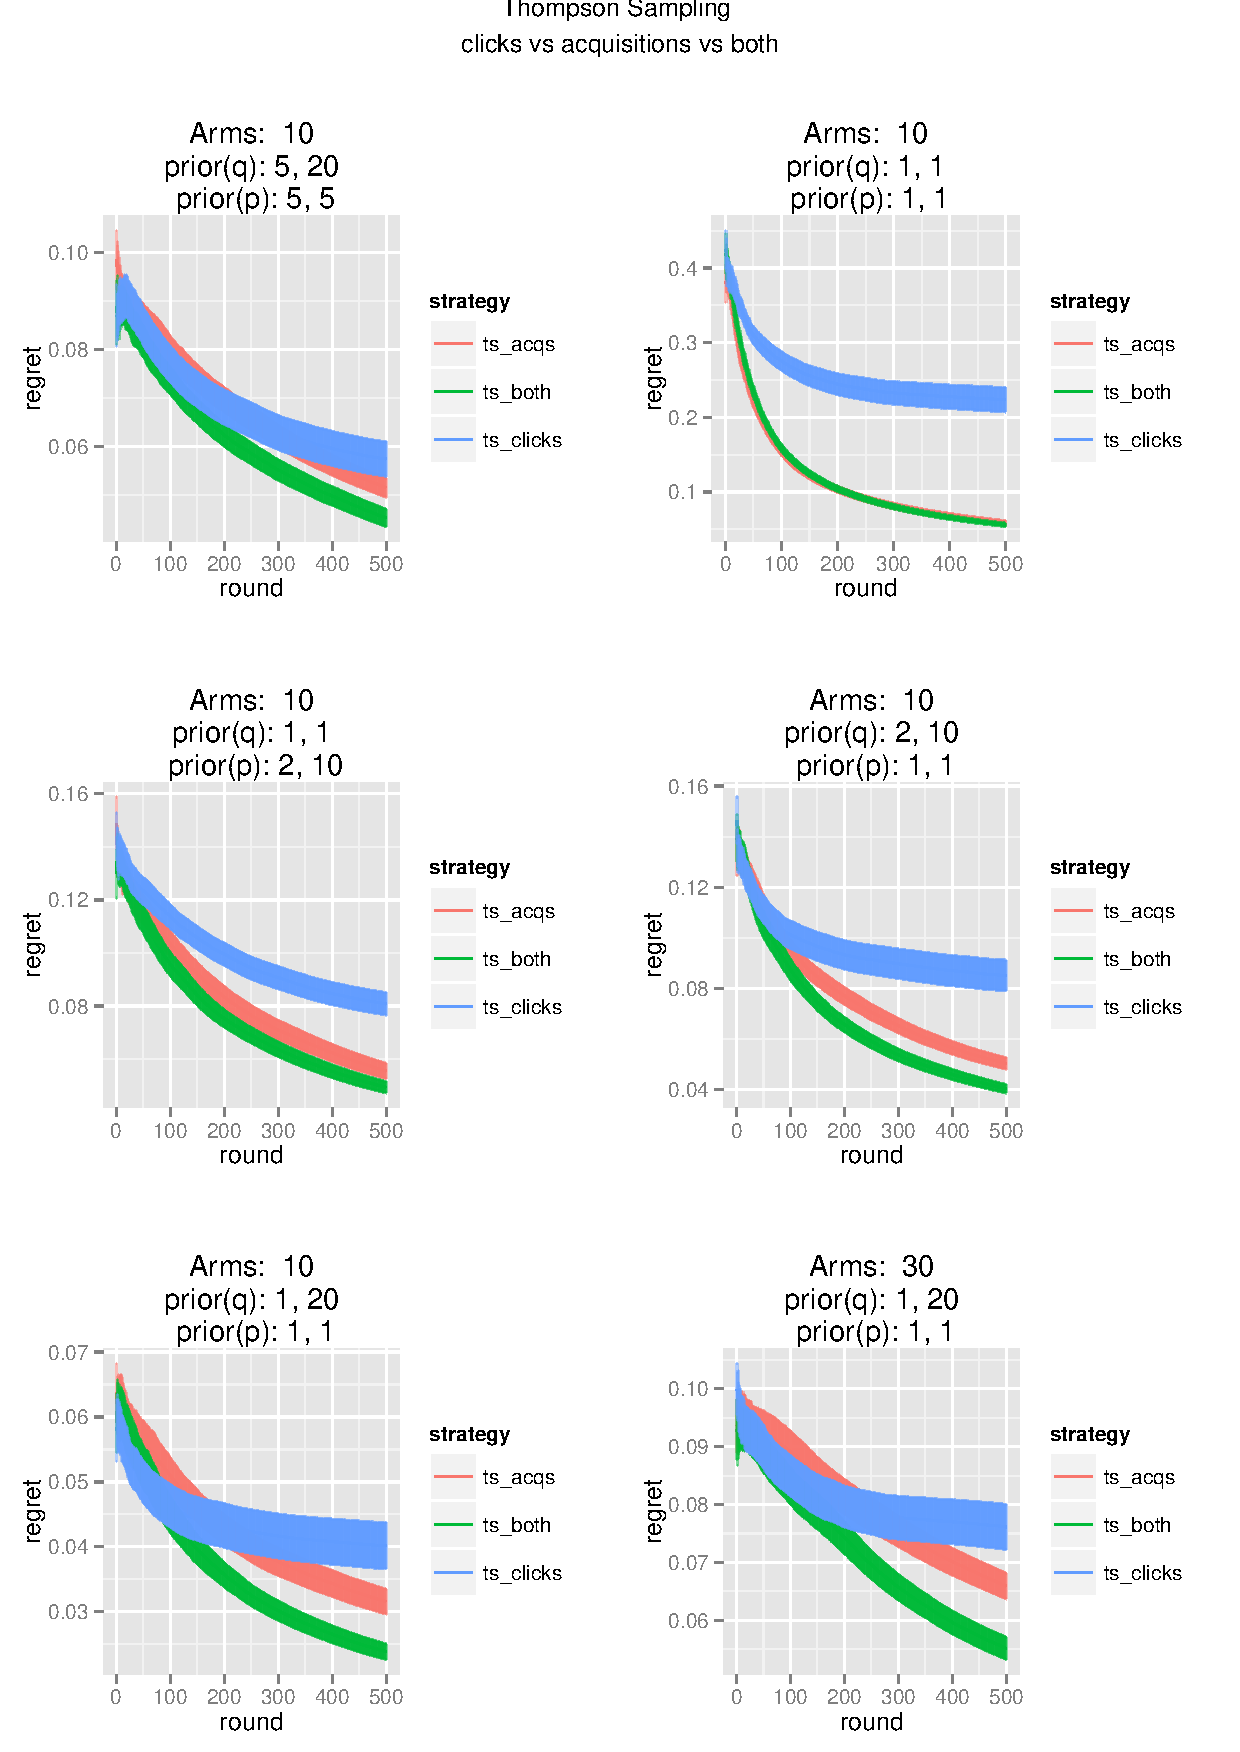
\includegraphics[scale=0.7]{P1to6.pdf}

\subsection{Discussion}

\begin{description}
	\item[ts clicks] typically reduces regret very quickly particularly with few arms and high variance on p. But over longer periods loses out to ts acqs and ts both since the best arm does not always have the highest rate of clicks. If there is a high variance on q, it can go very wrong.
	\item[ts acqs] performs well for long trials or where q can take on high values. But typically learns slowly, particularly when q has small values.
	\item[ts both] robust to the pathological cases that see poor performance from ts clicks and ts acqs, and in certain cases produced significantly improved results on both. In all but one instance (discussed next), ts both is at least as good as either algorithm.

\end{description}

We also note that ts clicks initially beats ts both, though this advantage goes away once the number of arms is increased. We hypothesise this is a feature of Thompson sampling rather than the model - by ignoring some of the uncertainty in the true value of r, ts clicks gains an early exploitation advantage.

We also note that as the number of arms goes up, the regret increases. This could be because the 'best arm' becomes further from the average arm given more arms, but possibly a sign of over-exploration.

We consider these are issues concerning the decision algorithm (Thompson sampling) in the next section.

\pagebreak

\section{Simulation testing - Bayes Adaptive policy}

In the previous section, we demonstrated that a more sophisticated model offered stronger inference and could reduce MAB regret. But we also noted a couple of instances where performance was not as good as it might be. 

With this in mind, we now look at options for decision algorithms. In particular we ask the question - given varying number of arms and campaign length, what is the best policy? 

PAC learning approaches look to limit the number of sub-optimal decisions (TODO add references). But this pure exploration approach does not naturally map to our goal of maximizing value from our campaign budget.

For given priors, it is possible to define a 'Bayes-optimal' policy. A MAB problem is a one state MDP with unknown payoffs. We can turn this in to a many state MDP with known payoff functions. Each state represents one possible value of the posterior. Each transition probability is given it's expected value based on the current posterior. This is called the Bayes Adaptive MDP. Now that we know the action rewards and transition probabilities, the optimal decision policy is provided by the Bellman equation from optimal control theory.

TODO - Reference Bayes Adaptive Reinforcement learning,
Optimal Adaptive Policies for Markov Decision Processes.

\subsection{Strategies}

TODO - add recursive definition for optimal arm aswell as how expectation is calculated from prior.

\begin{description}
	\item[ba both] Each arm is initialized with beta prior for both p and q. Arm with maximum Q value is always chosen, where multiple arms have same Q value, one is selected at random.
	\item[ba acqs] The strategy only looks at acquisitions per view, ignoring clicks. Since the Beta priors on p and q do not directly translate in to a Beta prior on r, we estimate the parameters of a Beta prior for r using the mean and variance of p and q. This new Beta prior is updated in the usual way with acquisitions and views. The arm selected is the one with maximum Q value.
\end{description}


\subsection{Bayes Adaptive policy illustration}

The graphs below provide a demonstration of this policy. In each graph, we see which arm choice is optimal as a function of rounds remaining. Note the high expectation arm is preferred for short campaigns the moves toward the higher variance arms as the time horizon increases. The 6 panes show one possible scenario play out as arms are chosen and posteriors are updated.

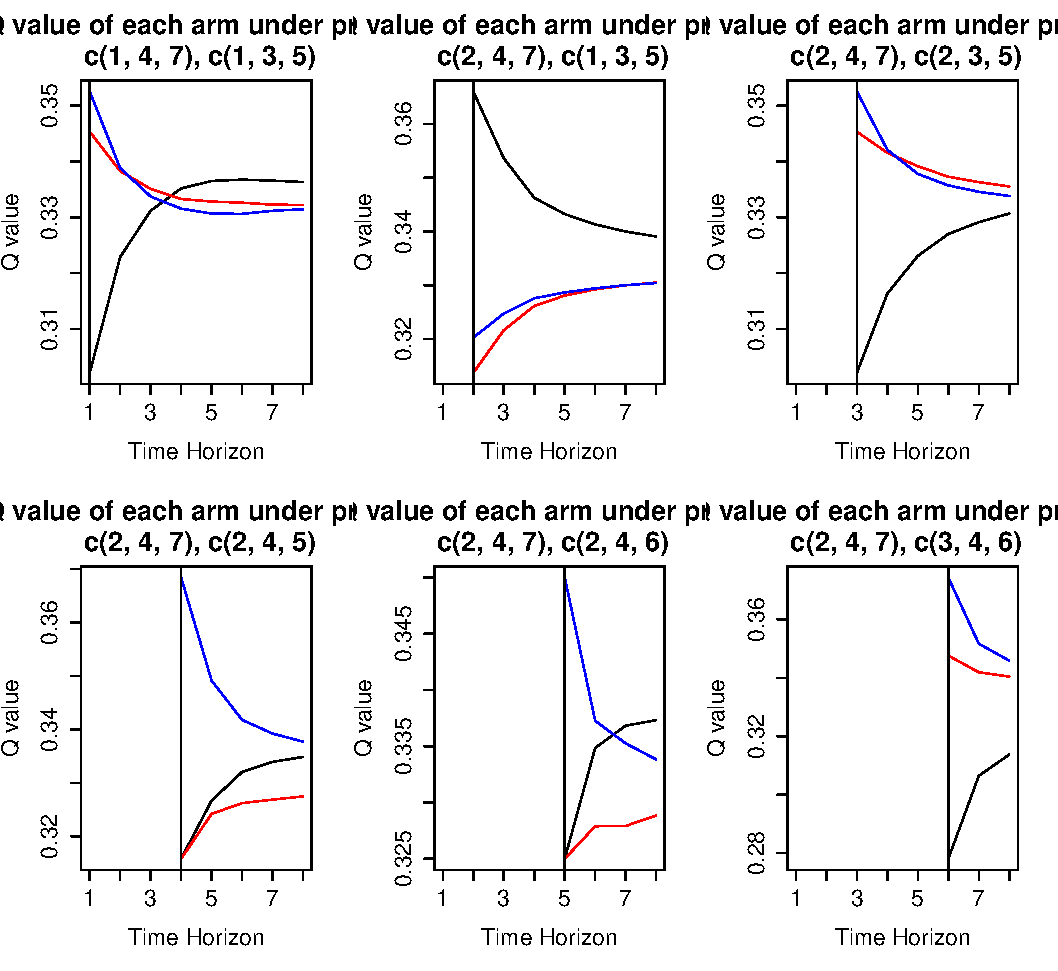
\includegraphics[scale=0.7]{BARLillustration.pdf}

This solution has a number of particularly attractive characteristics over probability matching strategies such as Thompson sampling and UCB:
\begin{itemize}
	\item We see that for small numbers of rounds, the algorithm purely exploits the high expectation arms, since there are too few rounds for the high variance arms to produce enough positive results to change our decisions. This is very relevant for our domain where we may have millions of arms (sites x placements x creatives x userType) but only a few 100,000 rounds and expectation of only a few 100 acquisitions. This addresses the issues we saw in previous section where the click only model would benefit from early exploitation of non-optimal arms. Thompson samply and UCB would typically over explore in these situations too.
	\item We can still integrate our prior information.
	\item If arms have some common dependency, such as using the same creative it understands there is greater exploration value.
	\item Policy responds to changes how we value events, underlying model, time horizons etc.
	\item The approach is orthogonal to the underlying model, so that we can develop the underlying model without needing to update the decision algorithm.
\end{itemize}

The limiting factor for this approach is that the algorithm has exponential order cost and so can be computed exactly only for small games. Various sampling based approximations exist \texttt{http://www.gatsby.ucl.ac.uk/~dayan/papers/guez\_jair2013.pdf}. 

\subsection{Results}

Using the same harness, we set up the experiment using a 'bayes-optimal' exploration algorithm. Due to the exponential order cost of this algorithm, we must keep the games to a small number of rounds. 

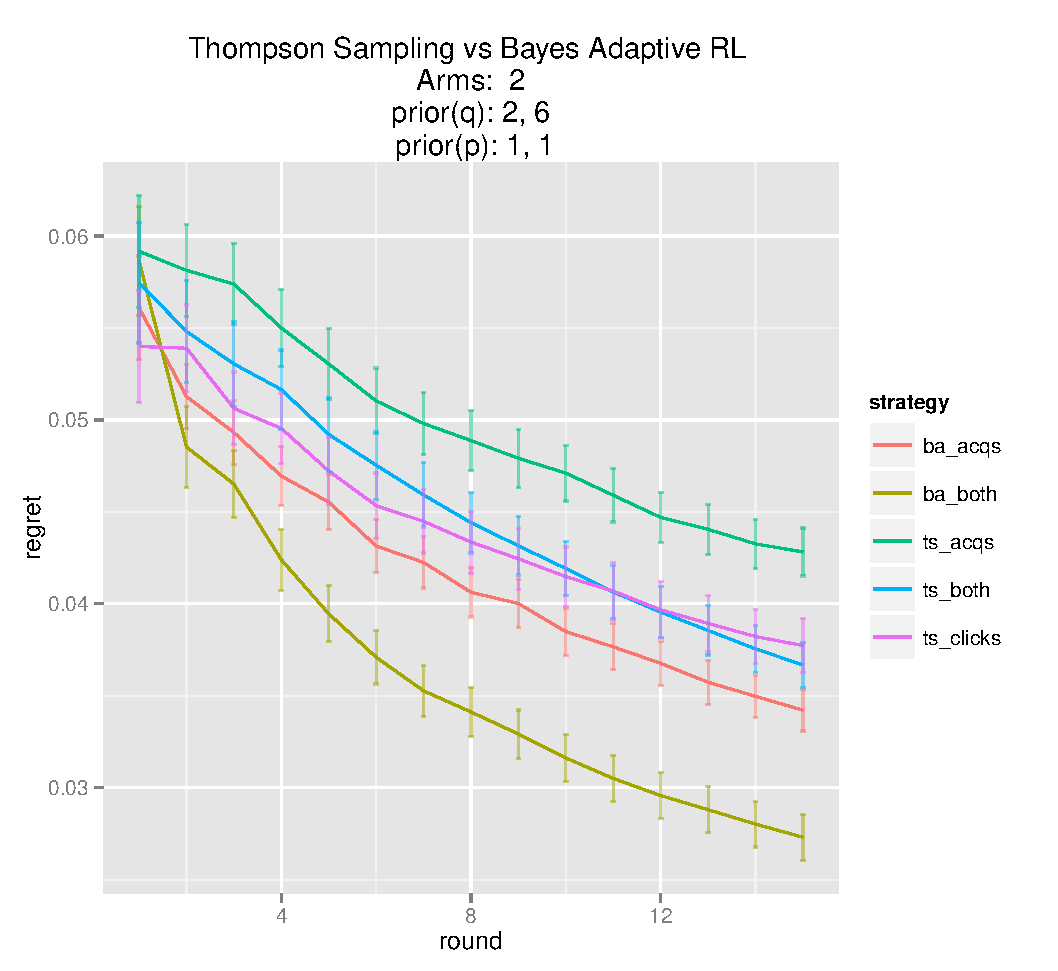
\includegraphics[scale=0.9]{TSvsBARL.pdf}

We see both Bayes Adaptive strategies improve on their Thompson Sampling equivalents. The strategy combining the improved model as well as the optimal decision policy offers very significant benefits.


\section{Scaling up}
Lai and Robbins ~\cite{lai1985asymptotically} proved that a class of decision algorithms meeting certain regret conditions were asymptotically optimal learners. This insight is the basis for the deterministic probability matching, UCB algorithms. 

We note that the optimal asymptotic regret leaves scope for a large constant regret term, as we found in our experiments poor performance over limited horizons.

We conjecture that due to the high number of arms, and low success rate, in practise we do not get to the region where asymptotic behaviour dominates.

The bayes-optimal solutions remain attractive. Although the Bellman equation gives us optimal solution, the computational time has order ${arms}^{rounds}$ and so becomes infeasible for large trials. We discuss the options providing similar results with less computation.
\section{Gittins Index}
Gittins ~\cite{gittins1979bandit} was able to show that the MAB problem with geometrically discounted regret could be treated as an index problem, very similar to job scheduling. The intuition here is that since playing one arm does not affect the rewards of other arms, a value can be computed using only information about that arm. The value is the expected ‘rate’ of reward under an optimal stopping rule.

The calculation of this index typically involves choosing a number of rounds to look ahead, the less the discount factor, the more rounds are required to get a close approximation. Then calculate the value at round N and use backwards induction to calculate the value for round 0.

Although the Gittins index is not optimal in the finite horizon case (the value of alternate arms changes as a result of the loss of 1 round), it is a very close approximation. Our testing (not presented) confirms this GI and BA strategies achieve near equal regret.

As the calculation involves only 1 arm, the computation for a game has order ${arms} .{rounds}^3$, with the potential to share results between arms. We present results comparing GI to TS strategies with arms = 10, rounds = 50. We use the exact method described in Gittins 1979. Note that since this is a finite horizon game, there is no loss of accuracy associated with calculating a finite number of rounds.

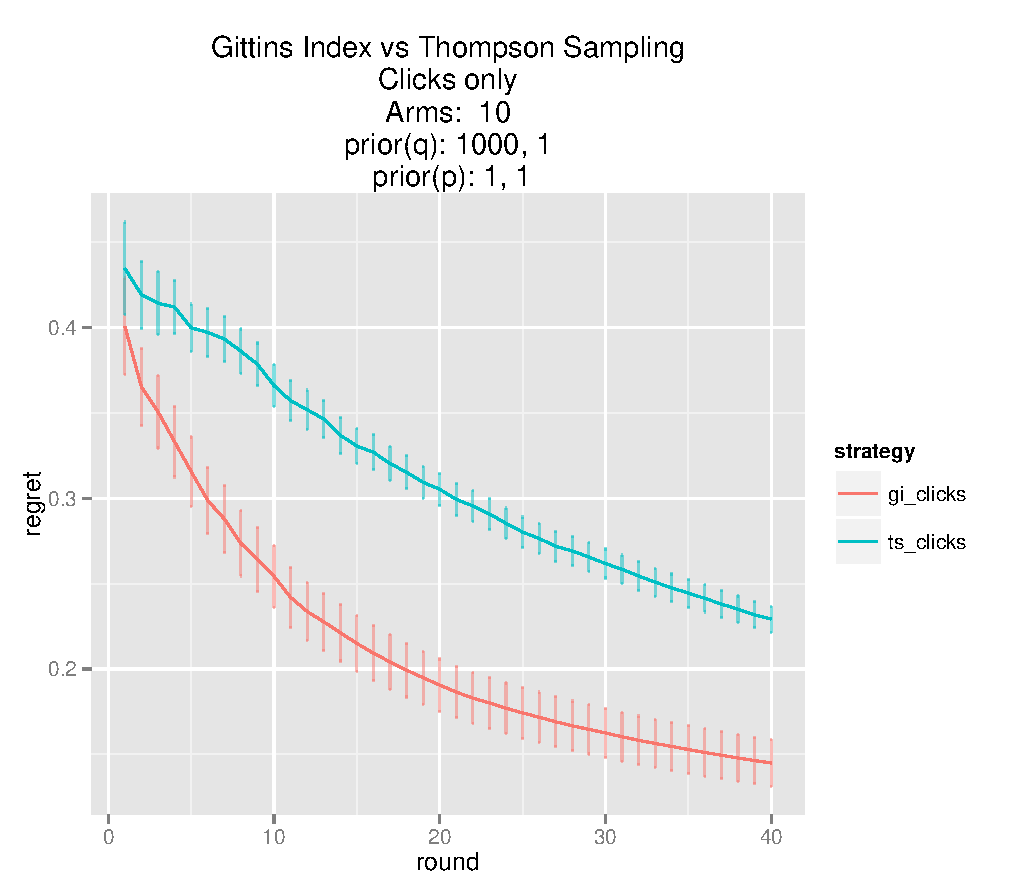
\includegraphics[scale=0.7]{GIvsTS.pdf}

We demonstrate in the appendix that it is simple to adapt the GI for binomial bandits to the ‘both’ model as it only requires taking expectations.

There are several methods looking for more computationally efficient calculation, the most popular being the ‘calibration method’ where a grid of candidate GI values is used to obviate the need to recurse. See Nino-Mora ~\cite{nino2011computing} for an overview. The cost for these methods is still of order at least $rounds^3$ (depending on matrix multiplication algorithm used) and so will not scale to say a million rounds.

Noting that GI is a function of only 5 variables, we consider approximations. Brezzi and Lai ~\cite{brezzi2002optimal} provide a closed form (i.e. constant order) solution to the infinite horizon problem using a Normal approximation by relating the discrete time problem to a continuous time Wiener process.  The same paper references Lai ~\cite{lai1987adaptive} for asymptotically optimal solutions for the finite horizon, undiscounted problem for single parameter exponential family distributions. Burnetas and Katehakis ~\cite{burnetas1996optimal} extend this to multiparameter univariate distributions.

The multiparameter solution would fit our 'both' model well and provide opportunity to extend the funnel to include additional intermediate steps. Unfortunately, as earlier noted, our testing finds these approaches do not work well with the arms, rounds and rates we work with.

\subsection{GI approximations}

There are several ways to reduce the computational cost due to the number of arms - grouping similar arms (e.g. contextual / factorial bandits ) or reuse of similar GI calcs. But the limiting issue is the cost due to large number of rounds.

Given that we are often working with very small rates, we might calculate GI by grouping the updates and enumerating only the more likely outcomes. For example, with a rate of 0.5\%, we might group by 1000 rounds and consider outcomes 0 to 12 which covers 0.998 of the distribution. 

\pagebreak

\section{Appendix}

\subsection{Do Clicks Matter}

\subsubsection{Distribution of a conditioned on n}

Firstly note that:

\begin{align}
{w+a \choose w}{n \choose w+a} &= \frac{n!}{(n-w-a)!w!a} \\
	&= \frac{n!(n-a)!}{((n-a)-w)!w!a!(n-a)!} \\
	&=  {n \choose a}{n-a \choose w}
\end{align}

We may construct the probability mass function for a using the conditional distributions:

\begin{align}
p(a|p,q,n) &= \sum_C p(a|q,c)p(c|p,n) \\
 &= \sum_{c=a}^n {c \choose a} p^a(1-p)^{c-a} {n \choose c} q^c (1-q)^{n-c}
\end{align}

Try to pull out a binomial by reparameterizing with $ w = c-a$:

\begin{align}
&= \sum_{w=0}^{n-a} {w+a \choose a} p^a(1-p)^w {n \choose w+a} q^{w+a} (1-q)^{n-w+a} \\
&= {n \choose a} (pq)^a \sum_{c=a}^n {n-a \choose w} ((1-p)q)^w (1-q)^{(n-a)-w} \\
&= {n \choose a} (pq)^a ((1-p)q +  (1-q))^{n-a} \\
&= Binom(a;pq,n)
\end{align}

Ref: http://math.stackexchange.com/questions/626457/conditional-binomials

\subsubsection{Posterior of qp}

We have now established that a is distributed as $Bin(qp,v)$. The question remains whether the uncertainty around the parameterization qp is reduced by modelling q and p separately.

For given a,c,n counts, p and q are independent of each other. If we assume a Haldane prior $\beta(0,0)$, we therefore describe their joint density as:

\begin{align}
 f_{P,Q}(p,q|a,c,n) = Beta(p;c,n-c) Beta(q;a,c-a)
\end{align}

Using the same approach as 'Rao, Linear Statistical Inference and its Applications, 3a.3, pg 168' to get the density of pq, apply the following transformation:
\begin{align}
 u(p,q) = qp, \quad v(p,q) = q  \\
 \implies p(u,v) = \frac{u}{v}, \quad q(u,v) = v
\end{align}

\begin{align}
 f_{U,V}(u,v) &= f_{P,Q}(p(u,v),q(u,v)) 
		\frac{\partial p \partial q}{\partial u \partial v} 
		\text{ ,in range }  (u<v<1,0<u<1) \\
 &= Beta(v;c,n-c) Beta(\frac{u}{v};a,c-a) v^{-1} \\
 &= k . v^{c-1} (1-v)^{n-c-1} (\frac{u}{v})^{a-1} (\frac{v - u}{v})^{c-a-1} v^{-1} \\
 &= k . (1-v)^{n-c-1} u^{a-1} (v - u)^{c-a-1}
\end{align}

Now integrate out v. Noting that the integral has the form of a Beta function, we shift and scale the integral with a change of variable.

\begin{align}
\text{Choose }  w &= \frac{v-u}{1-u} \\
f_U(u) &= k.u^{a-1} \int_u^1 (1-v)^{n-c-1} (v - u)^{c-a-1} \mathrm{d}v \\
 &= k.u^{a-1} \int_0^1 ((1-w)(1-u))^{n-c-1} (w(1-u))^{c-a-1} (1-u) \mathrm{d}w \\
 &= k.u^{a-1} (1-u)^{n-a-1} B(n-c,c-a) \\
 &= Beta(u;a,n-a) = Beta(qp;a,n-a) 
\end{align}

Thus showing that under the Haldane prior, click count does not change our estimation. By induction this can be extended to the product of any number of beta variables with appropriate parameters.

\subsubsection{Posterior of qp - with priors}

We now consider the form of the posterior under different possible priors:

\begin{align}
 f_{P,Q}(p,q|a,c,n) = Beta(p;c+\alpha_p,n-c+\beta_p) Beta(q;a+\alpha_q,c-a+\beta_q)
\end{align}

We can follow the calculation through to step (44) where the $v$ terms no longer cancel out:

\begin{align}
 k . v^{\alpha_p - \alpha_q - \beta_q}(1-v)^{n-c+\beta_p-1} u^{a+\alpha_q-1} (v - u)^{c-a+\beta_q-1}
\end{align}

We see that when $ \alpha_p = \alpha_q + \beta_q $ we will get a Beta form, but otherwise it is not analytic. 

\subsection{Bayed Adaptive MDP}

We show the Bayes Adaptive MDP for a 2 arm, 2 round game under the 'both' model. Each state, S, is defined by the 8-tuple of prior parameters, updated according to the outcome of each trial. From each state, we have the same control options - arm1 or arm2. There are three possible state transitions - no click, click but no acquisition, click and acquisition. The transition probabilities are the expectations, given the prior values. There is a payoff of 1 for transitions with an acquisition.

\begin{align}
s0 =
 \begin{pmatrix}
  \alpha_{p,1} & \beta_{p,1} & \alpha_{q,1} & \beta_{q,1} \\
  \alpha_{p,2} & \beta_{p,2} & \alpha_{q,2} & \beta_{q,2} 
 \end{pmatrix} \\
s1 =
  \begin{pmatrix}
   \alpha_{p,1}+1 & \beta_{p,1} & \alpha_{q,1}+1 & \beta_{q,1} \\
   \alpha_{p,2} & \beta_{p,2} & \alpha_{q,2} & \beta_{q,2} 
  \end{pmatrix} \\
s2 =
  \begin{pmatrix}
   \alpha_{p,1} & \beta_{p,1}+1 & \alpha_{q,1}+1 & \beta_{q,1} \\
   \alpha_{p,2} & \beta_{p,2} & \alpha_{q,2} & \beta_{q,2} 
  \end{pmatrix} \\
\vdots \\
s6 =
  \begin{pmatrix}
   \alpha_{p,1} & \beta_{p,1} & \alpha_{q,1} & \beta_{q,1} \\
   \alpha_{p,2} & \beta_{p,2} & \alpha_{q,2} & \beta_{q,2}+1 
  \end{pmatrix}
\end{align} 

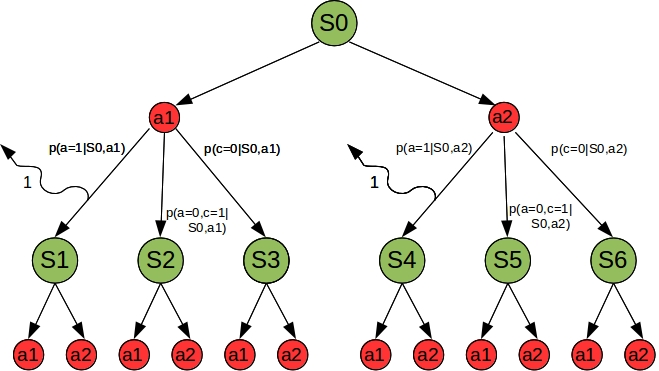
\includegraphics[scale=0.6]{BAMDP.jpg}

Note that although the posterior of pq does not have a closed form, it is still a cheap operation to take the expectation due to the independence of p and q. This means the both model is of similar order cost to the clicks-only or acquisitions-only model.

\begin{align}
	p(a=1|S,a1) = E[qp] = E[q]E[p] = 
		\left( \frac{ \alpha_{q,1} }{ \alpha_{q,1} + \beta_{q,1} } \right)
		\left( \frac{ \alpha_{p,1} }{ \alpha_{p,1} + \beta_{p,1} } \right) \\
	p(a=0,c=1|S,a1) = 
		\left( \frac{ \beta_{q,1} }{ \alpha_{q,1} + \beta_{q,1} } \right)
		\left( \frac{ \alpha_{p,1} }{ \alpha_{p,1} + \beta_{p,1} } \right) \\
	p(c=0|S,a1) = 
		\left( \frac{ \beta_{p,1} }{ \alpha_{p,1} + \beta_{p,1} } \right) 
\end{align}	

The optimal policy under this MDP is to greedily choose action with maximum value. The value for each of the 12 actions in the second round is simply the expected payoff $E[qp]$ given the state S1-S6 that the action is being taken from. The value of actions in the first round is the expectation of their immediate payoff, plus the expectation of the maximum value in the second round.

\subsection{Adaptation for Gittins index}

We can adapt the above MDP to calculate a Gittins index for arm 1. To do this, we replace arm 2 with a fixed (but unknown) payoff arm. We may then calculate the maximum possible payoff of arm 2 such that we both arms have equal value in the first round. This can be achieved by backwards induction.

\bibliography{refs}{}
\bibliographystyle{plain}

\end{document}
